\documentclass[conference]{IEEEtran}
\IEEEoverridecommandlockouts
% The preceding line is only needed to identify funding in the first footnote. If that is unneeded, please comment it out.
\usepackage{cite}
\usepackage{amsmath,amssymb,amsfonts}
\usepackage{algorithmic}
\usepackage{graphicx}
\usepackage{textcomp}
\usepackage{xcolor}

\graphicspath{ {./} }
\pagestyle{plain}
\def\BibTeX{{\rm B\kern-.05em{\sc i\kern-.025em b}\kern-.08em
    T\kern-.1667em\lower.7ex\hbox{E}\kern-.125emX}}
\begin{document}

\title{OpenDS: An Open Source Implementation of Discriminant Saliency on Center-surround Hypothesis\\
\thanks{A project proposal based on “On the plausibility of the discriminant center-surround hypothesis for visual saliency” by Dashan Gao; Vijay Mahadevan and Nuno Vasconcelos in 2008.}
}

\author{\IEEEauthorblockN{Yen Nhi Vuong}
\IEEEauthorblockA{\textit{EECS Department} \\
\textit{York University}\\
Toronto, Canada\\
ynhi97@my.yorku.ca}
}

\maketitle

\begin{abstract}
Most existing saliency detection models tend to target the high contrast in colors, intensity and orientation channels. However, it doesn’t accurately represent the visual focus of human. The saliency map most likely turns out to be a highlighted contour map of the image itself, rather than the actual focus point or region that people look at. In order to quantitatively predict human eye fixation on natural scenes, a research paper proposes saliency detection based on discriminant hypothesis. The discriminant saliency hypothesis is developed on top of the classical assumption that bottom-up saliency is a center-surround process. The methodology consists of two stages of detection, involving discriminant saliency detection, and leveraging natural image statistics to finally distinguish the target pop-out.
\end{abstract}

\begin{IEEEkeywords}
saliency, bottom-up, itti-koch, discriminant hypothesis, center-surround map
\end{IEEEkeywords}

\section{Introduction}
In computer vision, saliency is defined as standout part(s) of the image with distinct properties that draw eye fixation, which is the attention of the viewers. There are primary 2 saliency cues: \textit{bottom-up} - fast, stimulus-driven mechanism, and \textit{top-down} - slower, goal-driven mechanism [1]. Bottom-up saliency is more common in development as people tend to do it naturally without following certain tasks. Bottom-up is also highly desired because it allows us to understand what typically catches our attention, what visual features falls into the retina and so on...

The original research paper is called  \textit{"On the plausibility of the \textbf{discriminant center-surround hypothesis} for visual saliency”} by Dashan Gao. \textbf{Discriminant analysis} concerns with classifying set of observed data into predefined classes, giving minimum probability of expected error. The analysis requires a discriminant function. The \textbf{center-surround} hypothesis suggests bottom-up saliency as a center-surround process that derives optimal saliency architecture. In this architecture, saliency is detected from discriminating between the centre area of interest (\textit{the center}) and the neighbourhood surrounding it (\textit{the surround}) [2]. Optimal saliency detectors can serve psychophysics predictions of human saliency such as eye fixation prediction on natural scenes, background subtraction on high dynamic scenes and motion-based saliency in the presence of ego-motion [3]. 

This is an Engineering project which aims to reproduce the discriminant saliency model in Python 3 code with the help of open-source libraries such as OpenCV and Numpy.

\section{Methodology and Implementation}

\begin{figure*}[h]
    \centering
    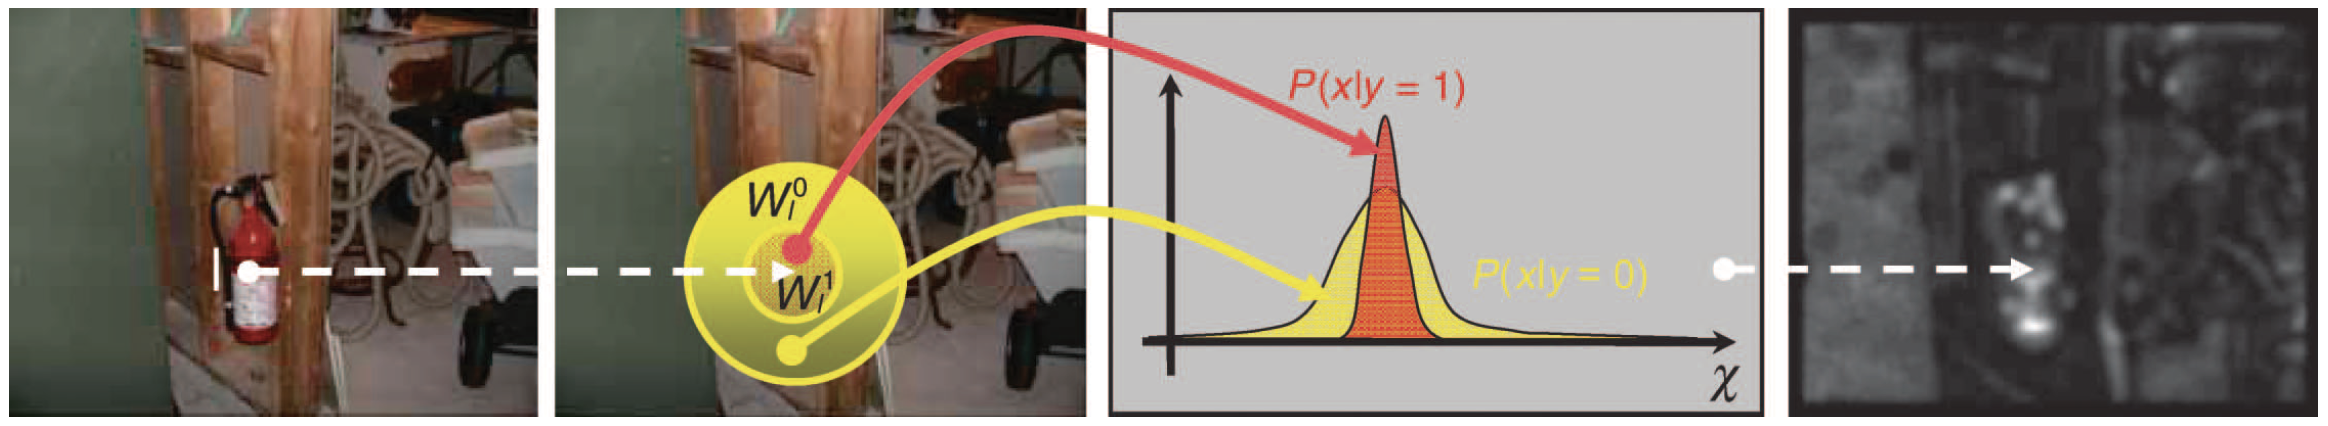
\includegraphics[width=7in]{research.png}
    \caption{ Illustration of discriminant center-surround saliency}
    \label{fig:centersurround}
\end{figure*}

The general architecture of image processing mainly follows the Itti-Koch-Niebur (IKN) model [6]. 

For static imagery, the process consists of 2 main stages. First stage is feature decomposition, using wavelet or Gabor decomposition to process into intensity map, and 4 color channels. The second stage is saliency detection which involves the center-surround classification (with provided formula for calculation) [7]. It also combines with Gabor or wavelet coefficients to reduce complexity of high dimensional image. One concern was to make sure OpenCV is able to handle the RGBY color channels and taken in account for visual angle (pixels/degrees). 

\begin{figure}[h]
    \centering
    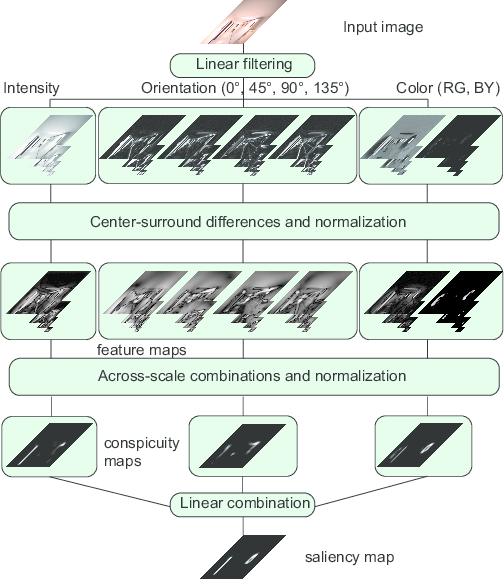
\includegraphics[width=3.3in]{itti.png}
    \caption{Itti-Koch model with center surround map computation}
    \label{fig:itti}
\end{figure}
 
\section{Results and Validation}
The project final step would be to apply the implemented model to a set of input images, which is preferably close to the research’s original test set. Previously, the researchers relied on classical experiments in visual attention which were both qualitative and quantitative. For simple target pop-out test, some example images were provided directly in the research paper. And to generate progressive/dependency graph between saliency versus image feature, more static and motion data will be needed. 

Due to the lack of test data sources, the project will simulate input images with similar features in such a way that if the model is computed correctly, the outcome should mimic the same behavior as the research results. Essentially it’s possible to use previous psychophysics results as a benchmark to evaluate the model. For more reliable online test set on saliency detection, some test input will be retrieved at the Toronto Dataset.

Neil Bruce, John K. Tsotsos. Attention based on information maximization.120 color images of outdoor and indoor scenes (size: 681 x 511px). Observers: 20 undergrads, grads. A large portion of images here do not contain particular regions of interest. Eye tracker: ERICA workstation including a Hitachi CCD camera with an IR emitting LED.

 
 
\section*{Acknowledgment}

The preferred spelling of the word ``acknowledgment'' in America is without 
an ``e'' after the ``g''. Avoid the stilted expression ``one of us (R. B. 
G.) thanks $\ldots$''. Instead, try ``R. B. G. thanks$\ldots$''. Put sponsor 
acknowledgments in the unnumbered footnote on the first page.

\section*{References}

Please number citations consecutively within brackets \cite{b1}. The 
sentence punctuation follows the bracket \cite{b2}. Refer simply to the reference 
number, as in \cite{b3}---do not use ``Ref. \cite{b3}'' or ``reference \cite{b3}'' except at 
the beginning of a sentence: ``Reference \cite{b3} was the first $\ldots$''

Number footnotes separately in superscripts. Place the actual footnote at 
the bottom of the column in which it was cited. Do not put footnotes in the 
abstract or reference list. Use letters for table footnotes.

Unless there are six authors or more give all authors' names; do not use 
``et al.''. Papers that have not been published, even if they have been 
submitted for publication, should be cited as ``unpublished'' \cite{b4}. Papers 
that have been accepted for publication should be cited as ``in press'' \cite{b5}. 
Capitalize only the first word in a paper title, except for proper nouns and 
element symbols.

For papers published in translation journals, please give the English 
citation first, followed by the original foreign-language citation \cite{b6}.

\begin{thebibliography}{00}
\bibitem{b1} G. Eason, B. Noble, and I. N. Sneddon, ``On certain integrals of Lipschitz-Hankel type involving products of Bessel functions,'' Phil. Trans. Roy. Soc. London, vol. A247, pp. 529--551, April 1955.
\bibitem{b2} J. Clerk Maxwell, A Treatise on Electricity and Magnetism, 3rd ed., vol. 2. Oxford: Clarendon, 1892, pp.68--73.
\bibitem{b3} I. S. Jacobs and C. P. Bean, ``Fine particles, thin films and exchange anisotropy,'' in Magnetism, vol. III, G. T. Rado and H. Suhl, Eds. New York: Academic, 1963, pp. 271--350.
\bibitem{b4} K. Elissa, ``Title of paper if known,'' unpublished.
\bibitem{b5} R. Nicole, ``Title of paper with only first word capitalized,'' J. Name Stand. Abbrev., in press.
\bibitem{b6} Y. Yorozu, M. Hirano, K. Oka, and Y. Tagawa, ``Electron spectroscopy studies on magneto-optical media and plastic substrate interface,'' IEEE Transl. J. Magn. Japan, vol. 2, pp. 740--741, August 1987 [Digests 9th Annual Conf. Magnetics Japan, p. 301, 1982].
\bibitem{b7} M. Young, The Technical Writer's Handbook. Mill Valley, CA: University Science, 1989.
\end{thebibliography}
\vspace{12pt}
\color{red}
IEEE conference templates contain guidance text for composing and formatting conference papers. Please ensure that all template text is removed from your conference paper prior to submission to the conference. Failure to remove the template text from your paper may result in your paper not being published.

\end{document}
